% figvirtualmemory.tex

\begin{figure}
\centering

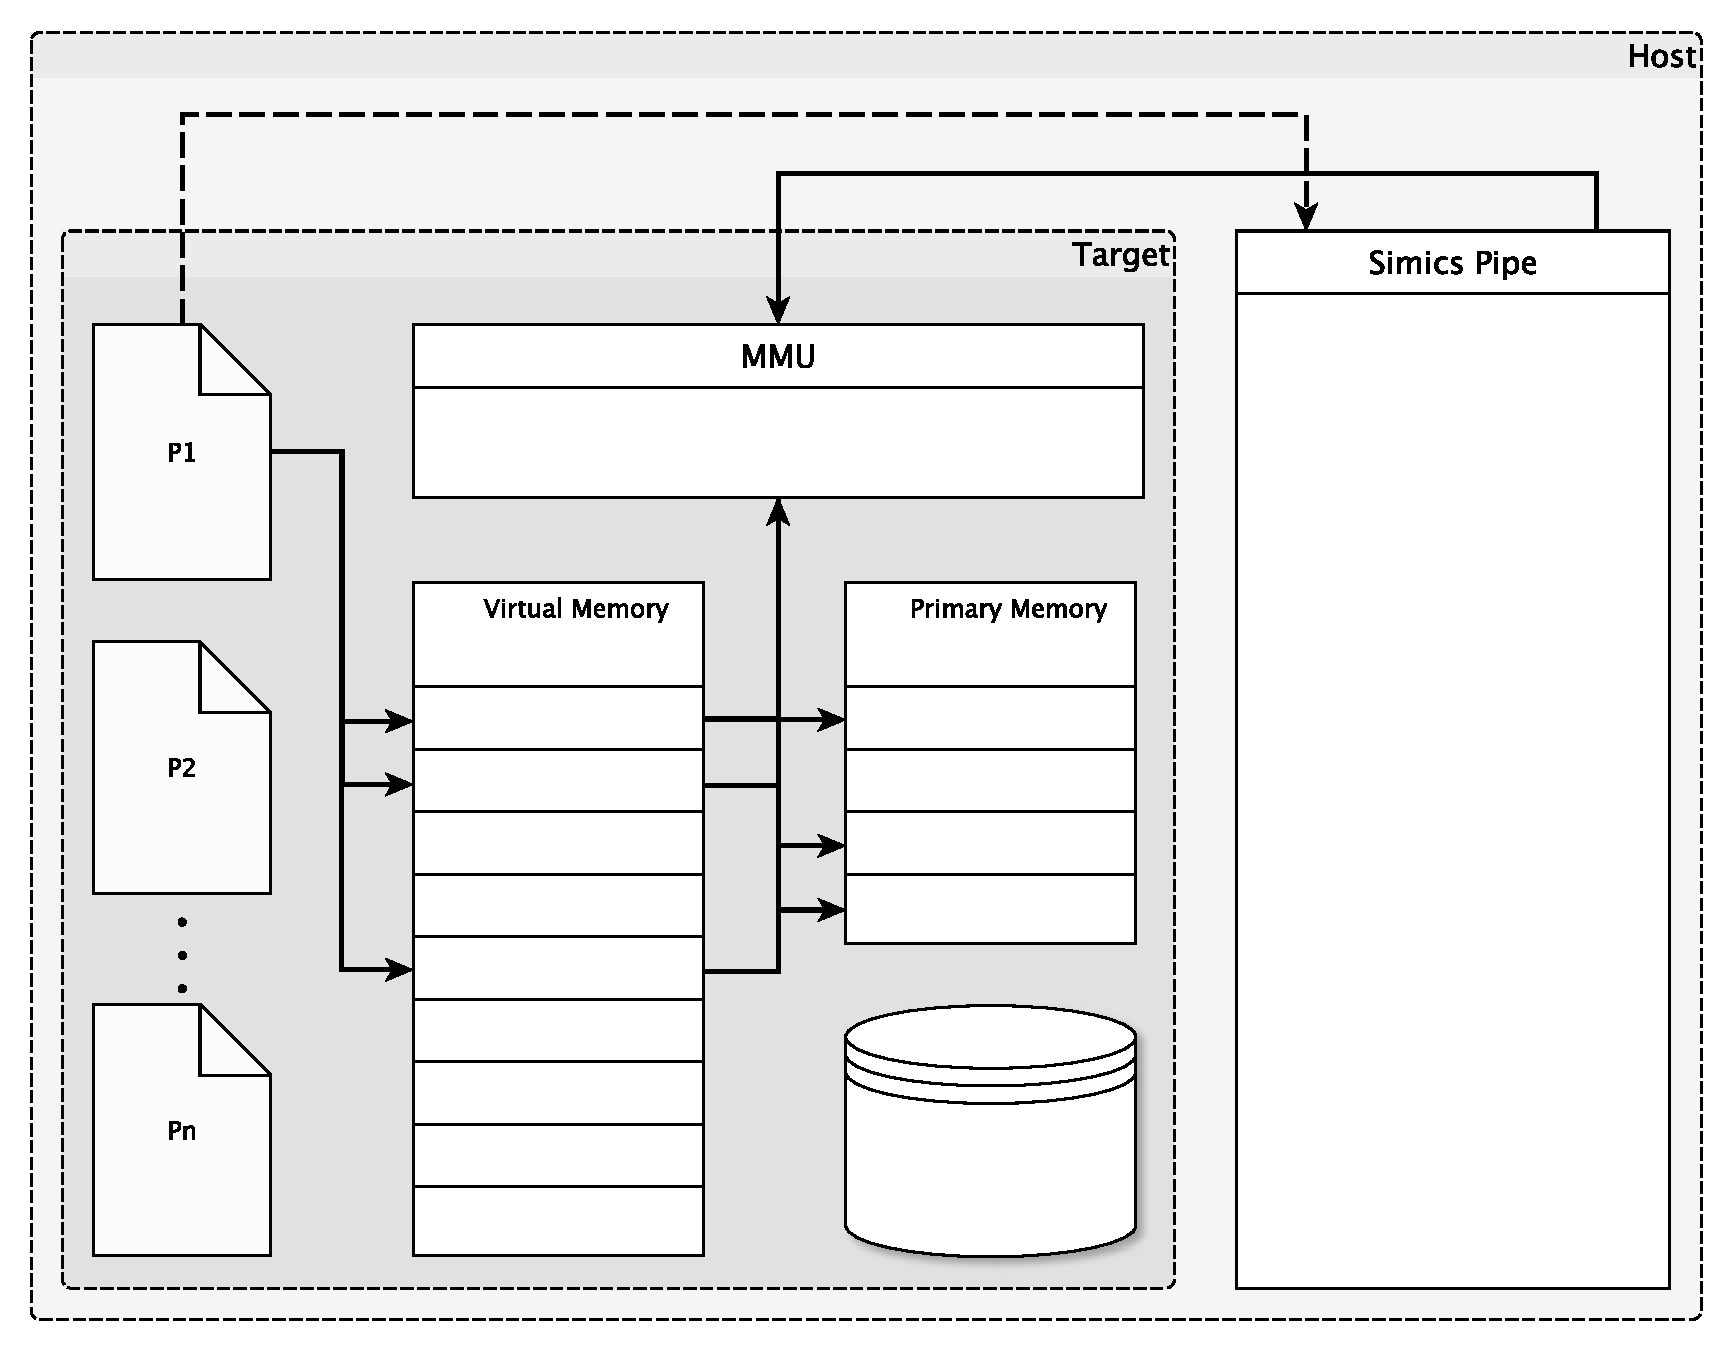
\includegraphics[width=\textwidth]{yedvirtualmemory.pdf}

\caption[Memory translation overview]{Memory translation overview. The OpenGL process hands a virtual memory address, pointing somewhere in the target system \textit{primary} memory, to the paravirtualized solution - which inquiries the target system MMU to retrieve designated bytestream directly from target physical memory.} % \footnote{Observe that said bytestream may not be present in secondary storage, due to memory page locking.}
\label{fig:virtualmemory}

\end{figure}